% Section 6.2, source PDF 78-90 / printed 68-80. Source-aligned staging, not yet accepted.
% block: exterior-calculus-section-heading page:78 type:section
\subsection{{Exterior calculus}}\label{sec:exterior-calculus}

% block: exterior-calculus-fields pages:78,79 type:ordinary-paragraph
{The primary objects of study in vector calculus are functions $\Omega\to\mathbb R$ and vector fields $\Omega\to\mathbb R^n$, defined on a domain $\Omega\subset\mathbb R^n$. In exterior calculus on $\mathbb R^n$, the primary objects are differential $k$-forms which are functions $\Omega\to\operatorname{Alt}^k\mathbb R^n$. In particular, the cases of functions and vector fields is included. Indeed, as we have seen, there are two different but natural ways to think of the functions of vector calculus as differential forms (either as $0$-forms or $n$-forms), and similarly vector fields may be identified with either $1$-forms or $(n-1)$-forms. This distinction, which is lost in vector calculus, turns out to be a strength of exterior calculus. Maxwell referred to it when he wrote that "physical vector quantities may be divided into two classes, in one of which the quantity is defined with reference to a line, while in the other the quantity is defined with reference to an area" \BookCite{58}. In higher dimensions other types of fields arise. For example, a differential $2$-form in four dimensions is a field with six independent components (the number of independent components in a $4\times4$ skew-symmetric matrix).}

% block: exterior-calculus-manifold-generality page:79 type:ordinary-paragraph
{Actually exterior calculus develops most naturally if we are more general, permitting as the domain $\Omega$ any manifold (finite dimensional, with or without boundary, and smooth enough that tangent spaces are defined), not just open subsets in $\mathbb R^n$. Much of the theory works in this degree of generality, depending only on the differentiable structure of the domain. Other concepts require additional structure: either an inner product (i.e., a Riemannian manifold), or an orientation (an oriented manifold), or both, and some formulas simplify if we use a preferred basis. Of course, a domain on $\mathbb R^n$ is endowed with all these things. But it is enlightening to hold clearly in mind what structures are required for what operations, as we shall do. From a practical point of view, even if we are only interested in solving boundary value problems in $\mathbb R^n$, we will need differential forms not only on the domain where the differential equation is defined but also on its boundary---which is a manifold, but not a domain in Euclidean space.}

% block: differential-forms-heading page:79 type:subsection
\subsubsection{{Differential forms}}\label{subsec:differential-forms}

% block: tangent-bundle-sections page:79 type:ordinary-paragraph
{Let $\Omega$ be a manifold of dimension $n$. At each point $x\in\Omega$, the tangent space $T_x\Omega$ is a vector space of dimension $n$, and the collection of all pairs $(x,v)$ with $x\in\Omega$ and $v\in T_x\Omega$ defines the tangent bundle, which is a manifold of dimension $2n$. A \emph{section} of this bundle is a function from $\Omega$ to its tangent bundle which assigns to each $x\in\Omega$ a tangent vector $v_x\in T_x\Omega$. That is, it is a tangent vector field.}

% block: differential-form-bundle page:79 type:ordinary-paragraph
{Applying the exterior algebra constructions of the previous section, we may define a bundle (the $k$th exterior power of the cotangent bundle) consisting of pairs $(x,\mu)$ with $\mu\in\operatorname{Alt}^kT_x\Omega$. A \emph{differential $k$-form} is a section of this bundle, i.e., a function which assigns to each $x\in\Omega$ an element of $\operatorname{Alt}^kT_x\Omega$. Thus $\omega$ being a differential $k$-form means that}
\[
\omega_x(v_1,\ldots,v_k)\in\mathbb R\quad\forall x\in\Omega,\ v_1,\ldots,v_k\in T_x\Omega,
\]
{with the dependence on the vectors $v_i$ being multilinear and alternating. We will usually require some degree of smoothness for the dependence on $x$, varying with the context. In the case where $\Omega$ is indeed a subdomain of $\mathbb R^n$, we may identify all the tangent spaces with $\mathbb R^n$, and so a differential $k$-form is just a function $\Omega\to\operatorname{Alt}^k\mathbb R^n$. It may be written as}
\begin{equation}\label{eq:differential-form-coordinates}
\omega=\sum_{1\leq\sigma_1<\cdots<\sigma_k\leq n}a_\sigma\,dx^{\sigma_1}\wedge\cdots\wedge dx^{\sigma_k},
\end{equation}
{with the coefficients $a_\sigma$ real-valued functions on $\Omega$.}

% block: differential-form-space-notation page:79 type:ordinary-paragraph
{We write $\Lambda^k(\Omega)$, or just $\Lambda^k$, for the vector space of differential $k$-forms on $\Omega$ when we do not need to emphasize the exact degree of smoothness expected. When we do, we will precede the notation with a function space. For example, $C\Lambda^k$ denotes the space of continuous differential forms, $C^1\Lambda^k$ of continuously differentiable forms, etc. We will introduce notation for spaces with different specified levels of smoothness below.}

% block: differential-form-pointwise-operations page:80 type:ordinary-paragraph
\medskip\noindent\textbf{{Exterior product, contraction, inner product, Hodge star, vector proxies}}\par
{The algebraic operations on alternating multilinear forms discussed in the previous section can be applied to differential forms pointwise. For example, the exterior product of $\omega\in\Lambda^j$ and $\mu\in\Lambda^k$ is a differential $(j+k)$-form given by}
\[
(\omega\wedge\mu)_x=\omega_x\wedge\mu_x.
\]
{Similarly, if $v$ is a vector field on $\Omega$ and $\omega\in\Lambda^k(\Omega)$, then $\omega\lrcorner v$ is a differential $(k-1)$-form. In order to extend the operations that need an inner product, we require the manifold $\Omega$ to be Riemannian, so that at each point $x$ there is given an inner product on $T_x\Omega$. The inner product should depend smoothly on $x$ in the sense that if $v_x$ and $w_x$ are smooth vector fields, then $x\mapsto\langle v_x,w_x\rangle_{T_x\Omega}$ should be a smooth function on $\Omega$ (the exact degree of smoothness again depending on the context). Several of the algebraic operations also require an orientation of the tangent spaces $T_x\Omega$ and we suppose that these have been assigned at each point in a consistent fashion. This requires that the manifold be orientable. It is not possible, for example, on a Möbius strip. On an oriented Riemannian manifold, there is a unique volume $n$-form, characterized by the fact that at each point $x$ it assigns the value $1$ to each positively oriented orthonormal basis of $T_x\Omega$. The Hodge star operator from $\Lambda^k$ to $\Lambda^{n-k}$ is then defined pointwise by \eqref{eq:hodge-star-characterization}, and we can compute the inner product in $L^2\Lambda^k(\Omega)$ by}
\[
\langle\omega,\nu\rangle_{L^2\Lambda^k}=\int_\Omega\langle\omega,\nu\rangle\operatorname{vol}=\int_\Omega\omega\wedge\star\nu,\qquad\omega,\nu\in L^2\Lambda^k(\Omega).
\]
{Applying the vector proxies pointwise, we can identify differential $0$-forms and differential $n$-forms with real-valued functions on the manifold and identify differential $1$-forms and differential $(n-1)$-forms with tangential vector fields.}

% block: smooth-pullback page:80 type:ordinary-paragraph
\begingroup\emergencystretch=1em
\medskip\noindent\textbf{{Pullback under smooth maps and traces}}\par
{If $\phi:M\to N$ is a differentiable map between manifolds, its derivative $\phi'(x)$ is a linear map of $T_xM$ to $T_{\phi(x)}N$. If $\omega\in\Lambda^k(N)$, we may therefore define a differential $k$-form on $\Omega$ by}
\begin{equation}\label{eq:smooth-pullback-definition}
(\phi^*\omega)_x=\phi'(x)^*\omega_{\phi(x)},
\end{equation}
{where, on the right-hand side, we are using the algebraic pullback defined by \eqref{eq:linear-pullback-definition}. This defines the pullback $\phi^*\omega\in\Lambda^k(M)$ of a differential form under a smooth map. As in the algebraic case, pullback acts contravariantly and respects the exterior product.}

\par\endgroup
% block: differential-trace-proxies pages:80,81 type:ordinary-paragraph
{The pullback of the inclusion of a submanifold $M$ into another manifold $N$ is called the trace operator, denoted $\operatorname{tr}:\Lambda^k(N)\to\Lambda^k(M)$. In the case of $0$-forms it is just restriction of functions. The derivative of the inclusion at a point $x\in M$ is the inclusion of $T_xM\subset T_xN$. This fact and our calculations at the end of Section~\ref{subsec:alternating-form-operations} provide formulas for the trace in terms of proxies in two important cases. If $w$ is a vector field on $N$ corresponding to some $1$-form $\omega\in\Lambda^1(N)$, then the vector field $\bar w$ on $M$ corresponding to $\operatorname{tr}\omega\in\Lambda^1(M)$ is given by}
\[
\bar w(x)=\pi w(x),\qquad x\in M,
\]
{where $\pi=\pi_{T_xM}:T_xN\to T_xM$ is the orthogonal projection. If instead $\dim M=\dim N-1$ and the vector field $w$ corresponds to $\omega\in\Lambda^{\dim N-1}(N)$, then $\operatorname{tr}\omega$ corresponds to the scalar function $\langle w,n\rangle$ on $M$, where $n$ is the appropriately oriented unit normal to $M$ in $N$.}

% block: coordinate-trace page:81 type:ordinary-paragraph
{In the case $M=\mathbb R^{n-1}$, $N=\mathbb R^n$, with the inclusion given by $x\mapsto(0,x)$, we can write the corresponding trace operator in terms of coordinates. If $\omega$ is the differential form given by \eqref{eq:differential-form-coordinates}, then}
\begin{equation}\label{eq:differential-trace-coordinates}
\operatorname{tr}\omega=\sum_{\{\sigma\mid\sigma_1>1\}}(\operatorname{tr}a_\sigma)\,dx^{\sigma_1}\wedge\cdots\wedge dx^{\sigma_k}.
\end{equation}
{The trace operator appearing in the term $\operatorname{tr}a_\sigma$ on the right-hand side is the $0$-form trace, which is just the restriction to $\mathbb R^{n-1}$.}

% block: exterior-derivative-heading page:81 type:subsection
\subsubsection{{Exterior derivative}}\label{subsec:exterior-derivative}

% block: exterior-derivative-definition page:81 type:ordinary-paragraph
{The exterior derivative, which maps $\Lambda^k(\Omega)$ to $\Lambda^{k+1}(\Omega)$, is the fundamental operator of exterior calculus. It is simplest to define when $\Omega$ is a domain in $\mathbb R^n$. If $\omega$ is a smooth differential $k$-form, and $v_1,\ldots,v_k$ are $k$ vectors in $\mathbb R^n$, then $\omega_x(v_1,\ldots,v_k)$ is a differentiable function of $x$, which is alternating multilinear in the $k$ vectors. If $v_0$ is an additional vector, then we may apply $\partial_{v_0}:=v_0\cdot\operatorname{grad}$, the directional derivative in the direction $v_0$, to this function, obtaining a quantity which depends on $x$ and all $(k+1)$-vectors. The dependence on the vectors is linear in each but is not alternating. To get a $(k+1)$-form we take the alternating part. Multiplying this by $k+1$ gives the exterior derivative $d\omega$:}
\[
(d\omega)_x(v_0,\ldots,v_k)=\sum_{j=0}^k(-)^j\partial_{v_j}\omega_x(v_0,\ldots,\widehat{v_j},\ldots,v_k).
\]

% block: exterior-derivative-coordinates page:81 type:ordinary-paragraph
{Written in terms of the standard coordinates on $\mathbb R^n$, a general element of $\Lambda^k(\Omega)$ can be written as}
\[
\omega=\sum_{1\leq\sigma_1<\cdots<\sigma_k\leq n}f_\sigma\,dx^{\sigma_1}\wedge\cdots\wedge dx^{\sigma_k},
\]
{where the coefficients $f_\sigma$ are functions on $\Omega$. Then}
\begin{equation}\label{eq:exterior-derivative-coordinates}
d\omega=\sum_\sigma\sum_{j=1}^n\frac{\partial f_\sigma}{\partial x^j}\,dx^j\wedge dx^{\sigma_1}\wedge\cdots\wedge dx^{\sigma_k}.
\end{equation}

% block: exterior-derivative-vector-calculus page:81 type:ordinary-paragraph
{In the case $k=0$, for example, we have the formula}
\[
df=\sum_{j=1}^n\frac{\partial f}{\partial x^j}\,dx^j.
\]
{Identifying the $1$-form on the right-hand side with a vector field, we see that the exterior derivative on a $1$-form on $\mathbb R^n$ is just the gradient operator. Similar considerations show that the exterior derivative on an $(n-1)$-form can be identified with the divergence operator. In three dimensions, the exterior derivative on $1$-forms can be viewed as a mapping from vector fields to vector fields and is found to be the curl operator. Thus, in this case the entire de Rham complex \eqref{eq:differential-forms-de-rham-complex} can be expressed in the terminology of vector calculus as in \eqref{eq:vector-calculus-de-rham-complex}.}

% block: exterior-derivative-pullback-invariance page:82 type:ordinary-paragraph
{An important property of the exterior derivative is that it is invariant under pullback. If $\phi:\Omega\to M$ is a map from a subdomain of $\mathbb R^n$ to a subdomain of $\mathbb R^m$, and $\omega\in\Lambda^k(M)$, then $\phi^*\omega\in\Lambda^k(\Omega)$ and}
\begin{equation}\label{eq:exterior-derivative-pullback}
d\phi^*\omega=\phi^*d\omega.
\end{equation}
{In the case where $\phi$ is a diffeomorphism between two domains of equal dimension, we conclude that}
\begin{equation}\label{eq:exterior-derivative-chart-definition}
d\omega=(\phi^{-1})^*d\phi^*\omega.
\end{equation}
{We may use this formula to define $d\omega$ when $M$ is a manifold rather than a domain in Euclidean space. We choose any chart $\phi$ mapping some $\Omega\subset\mathbb R^n$ onto an open set of $M$ and then use the formula \eqref{eq:exterior-derivative-chart-definition} to define $d\omega$ on that open subset. Since $M$ is covered by charts, in this way we define $d\omega\in\Lambda^k(M)$. That the definition does not depend on the choice of charts follows from \eqref{eq:exterior-derivative-pullback}. Moreover this invariance under pullback holds for any smooth maps between manifolds.}

% block: exterior-differential-leibniz page:82 type:ordinary-paragraph
{Another essential property of the exterior derivative is that it is a differential in the sense that $d\circ d=0$. It is enough to verify this on a domain in $\mathbb R^n$, where it follows easily from \eqref{eq:exterior-derivative-coordinates} thanks to the commutativity of partial derivatives. Equally essential is the Leibniz rule}
\begin{equation}\label{eq:exterior-leibniz-rule}
d(\omega\wedge\mu)=d\omega\wedge\mu+(-)^k\omega\wedge d\mu,\qquad\omega\in\Lambda^k(\Omega),\ \mu\in\Lambda^j(\Omega).
\end{equation}
{It is worth emphasizing that the exterior derivative is defined without any reference to an inner product (metric) or an orientation on the manifold. A differential $k$-form on any manifold can be differentiated to give a differential $(k+1)$-form.}

% block: differential-form-integration-heading page:82 type:subsection
\subsubsection{{Integration of differential forms}}\label{subsec:differential-form-integration}

% block: integration-orientation page:82 type:ordinary-paragraph
{A differential $k$-form can be integrated over an oriented $k$-dimensional manifold to give a real number. Notice that the form degree and the manifold dimension must be the same. No metric or measure is required on the manifold to define the integral, and if they exist, then the integral is independent of them. However, the orientation does matter. If we switch it, the sign of the integral changes.}

% block: integration-parallelepiped-definition page:82 type:ordinary-paragraph
{To get a basic idea of how the integral is defined, consider a parallelepiped $P$ determined by a point $x\in\mathbb R^k$ and $k$ linearly independent vectors $v_1,\ldots,v_k$, as in Figure~\ref{fig:integration-parallelograms}(a). If $\omega$ is a constant $k$-form on $P$, then the integral of $\omega$ over $P$ is simply $\omega_x(v_1,\ldots,v_k)$. If $\omega$ is smooth, but not constant, then this will be a good approximation of the integral if the parallelepiped is sufficiently small. Now any manifold can be approximated arbitrarily well by a collection of small tangent parallelopideds using coordinate charts, as illustrated in Figure~\ref{fig:integration-parallelograms}(b). We then get an approximate value for the integral by evaluating $\omega$ on each parallelogram and adding}
\[
\int_\Omega\omega\approx\sum_i\omega_{x^{(i)}}(v_1^{(i)},\ldots,v_n^{(i)}),
\]
{where the $x^{(i)}$ and $v_j^{(i)}$ are the points and tangent vectors determining the parallelograms. Passing to the limit we obtain $\int_\Omega\omega$.}

% block: integration-parallelograms-figure page:83 type:figure
\begin{figure}[htbp]\centering
\includegraphics[page=83,trim=102bp 494bp 52bp 62bp,clip,width=.90\linewidth]{../input/source/Finite Element Exterior Calculus.pdf}
\caption{{(a) A parallelogram determined by a point and two tangent vectors at the point. (b) A two-dimensional manifold can be approximated arbitrarily closely by a collection of tangent parallelograms.}}\label{fig:integration-parallelograms}
\end{figure}

% block: integration-diffeomorphism-invariance page:83 type:ordinary-paragraph
{One easy consequence of the definition is that the integral is invariant under orientation-preserving diffeomorphisms. That is, if $\phi:M\to N$ is such a diffeomorphism of $n$-dimensional manifolds, then}
\begin{equation}\label{eq:integration-pullback-invariance}
\int_M\phi^*\omega=\int_N\omega,\qquad\omega\in\Lambda^n(N).
\end{equation}
{In particular, we may use charts to reduce the computation of the integral over a manifold to integrals over subdomains of $\mathbb R^n$, and most of its properties can be verified in this way. If $\Omega$ is such a domain, then an $n$-form on $\Omega$ can be written $f(x^1,\ldots,x^n)\,dx^1\wedge\cdots\wedge dx^n$, and its integral is exactly what the notation}
\[
\int_\Omega f(x^1,\ldots,x^n)\,dx^1\wedge\cdots\wedge dx^n
\]
{suggests (i.e., it equals the Lebesgue integral of the function $f$ over $\Omega$). More generally, if $\Omega$ is an oriented Riemannian manifold, then $\int_\Omega f\operatorname{vol}$ coincides with the integral of $f$ with respect to its associated Riemannian measure.}

% block: integration-over-submanifold page:83 type:ordinary-paragraph
{If $\omega$ is a $k$-form on an $n$-dimensional manifold $\Omega$, and $M$ is an oriented $k$-dimensional submanifold of $\Omega$, then the trace of $\omega$ on $M$ is a $k$-form on a $k$-dimensional manifold and so can be integrated over $M$. Technically, the result should be written as $\int_M\operatorname{tr}_M\omega$, but frequently one just writes $\int_M\omega$. For example, suppose $M$ is an oriented curve in some domain in $\mathbb R^n$ and $\omega$ is a $1$-form on the domain. We may view $\omega$ as a vector field, and then $\operatorname{tr}_M\omega$ corresponds to the tangential projection of the vector field onto the curve. Thus $\int_M\omega$ is the usual line integral from vector calculus.}

% block: stokes-integration-by-parts-heading page:83 type:subsection
\subsubsection{{Stokes theorem and integration by parts}}\label{subsec:stokes-integration-by-parts}

% block: stokes-theorem page:83 type:ordinary-paragraph
{The capstone of exterior calculus is the Stokes theorem, a far-ranging generalization of the fundamental theorem of calculus. Under relatively mild smoothness requirements on the compact oriented $n$-dimensional manifold with boundary $\Omega$ and the differential form $\omega$ it states that}
\[
\int_\Omega d\omega=\int_{\partial\Omega}\operatorname{tr}\omega,\qquad\omega\in\Lambda^{n-1}(\Omega).
\]

% block: stokes-boundary-orientation page:84 type:ordinary-paragraph
{Again, the result is usually stated without writing the trace operator explicitly. The boundary orientation is inherited from that of the manifold (namely, a positively oriented basis for the tangent space of the boundary at some point is one which, when prepended by the outward normal at the point, is positively oriented for $\Omega$).}
{If we replace $\omega$ by $\omega\wedge\mu$ in this equation and use the Leibniz rule \eqref{eq:exterior-leibniz-rule} we obtain an integration-by-parts formula:}
\begin{equation}\label{eq:differential-forms-integration-by-parts}
\begin{gathered}
\int_\Omega d\omega\wedge\mu=(-)^{k+1}\int_\Omega\omega\wedge d\mu+\int_{\partial\Omega}\operatorname{tr}\omega\wedge\operatorname{tr}\mu,\\
\omega\in\Lambda^k(\Omega),\ \mu\in\Lambda^{n-k-1}(\Omega),
\end{gathered}
\end{equation}
{valid for sufficiently smooth forms (we shall investigate the required smoothness below). Using the Hodge star operator on the boundary, the boundary integral can be written as the inner product $\langle\star\operatorname{tr}\omega,\operatorname{tr}\mu\rangle_{L^2\Lambda^{n-k-1}(\partial\Omega)}$.}

% block: piola-application-heading page:84 type:subsection
\subsubsection{{An example application}}\label{subsec:piola-application}

% block: piola-application-derivation page:84 type:ordinary-paragraph
{Before continuing, we use the exterior calculus framework to derive a result of vector calculus that plays a large role in the development of mixed finite elements. (See, e.g., [\BookNumber{19}, Lemma 2.1.6] for a statement of the result in two dimensions.) Let $p:\Omega\to\mathbb R$ and $v:\Omega\to\mathbb R^3$ be scalar and vector fields on a domain $\Omega$ in $\mathbb R^3$, and consider the inner product $(p,\operatorname{div}v)_{L^2(\Omega)}$. Recognizing the divergence as the exterior derivative of a $2$-form, we let $\nu=v^1dx^2\wedge dx^3-v^2dx^1\wedge dx^3+v^3dx^1\wedge dx^2$ be the differential $2$-form with vector proxy $v$. Then $d\nu=(\operatorname{div}v)\operatorname{vol}$ and $(p,\operatorname{div}v)_{L^2(\Omega)}=\int_\Omega p\wedge d\nu$, where the integral on the right-hand side is in the sense of differential forms. Next, we suppose that $\phi:\widehat\Omega\to\Omega$ is an orientation-preserving diffeomorphism and apply invariance under pullback of the integral \eqref{eq:integration-pullback-invariance}, the exterior product \eqref{eq:linear-pullback-wedge}, and the exterior derivative \eqref{eq:exterior-derivative-pullback} to transform the integral over $\Omega$ to one over $\widehat\Omega$:}
\[
\int_\Omega p\wedge d\nu=\int_{\widehat\Omega}\phi^*(p\wedge d\nu)=\int_{\widehat\Omega}\phi^*p\wedge\phi^*d\nu=\int_{\widehat\Omega}\phi^*p\wedge d\phi^*\nu.
\]
{From the definition \eqref{eq:smooth-pullback-definition} for the pullback of a field and the formulas given at the bottom of Table~\ref{tab:exterior-algebra-r3} for the pullback of a linear map, we see that $\phi^*p=\hat p:=p\circ\phi$ and the proxy field for $\phi^*\nu$ is the vector field}
\[
\hat v=(\det\phi')(\phi')^{-1}(v\circ\phi):\widehat\Omega\to\mathbb R^3.
\]
{The vector field $\hat v$ is called the \emph{Piola transform} of $v$. We see that the Piola transform arises naturally as the pullback on $2$-forms and that, as a consequence, it satisfies the crucial property}
\[
(p,\operatorname{div}v)_{L^2(\Omega)}=(\hat p,\operatorname{div}\hat v)_{L^2(\widehat\Omega)}.
\]

% block: differential-forms-l2-heading page:84 type:subsection
\subsubsection{{The $L^2$ theory of differential forms}}\label{subsec:differential-forms-l2-theory}

% block: differential-forms-l2-introduction page:84 type:ordinary-paragraph
{In this section we suppose that $\Omega$ is a smooth compact $n$-dimensional oriented Riemannian manifold with or without boundary and we view the exterior derivatives $d=d^k$ as closed densely defined unbounded operators from $L^2\Lambda^k(\Omega)$ to $L^2\Lambda^{k+1}(\Omega)$ which fit together to create the $L^2$ de Rham complex. We show that the exterior derivative operators all have closed range and compute their adjoints.}

% block: l2-techniques-and-inner-product page:85 type:ordinary-paragraph
{The techniques are completely parallel to those used in Section~\ref{sec:vector-operators-adjoints} for the special case of a domain in $\mathbb R^3$.}

{Since we assume that an orientation and a Riemannian structure are given, the Hodge star is well-defined. From \eqref{eq:hodge-star-inner-product}, the $L^2$ inner product of the two $k$-forms is}
\[
\langle\omega,\mu\rangle_{L^2\Lambda^k}=\int_\Omega\langle\omega,\mu\rangle\operatorname{vol}=\int_\Omega\omega\wedge\star\mu,\qquad\omega,\mu\in\Lambda^k(\Omega).
\]
{We may drop the $\Lambda^k$ from the subscript on the inner product or drop the subscript altogether when there is little risk of confusion.}

% block: codifferential-definition page:85 type:ordinary-paragraph
{The \emph{codifferential} operator is defined as $\delta=\pm\star d\star$. The sign is determined by requiring that $\delta=\delta^k:\Lambda^k\to\Lambda^{k-1}$ satisfy}
\[
\star\delta\omega=(-)^kd\star\omega,\qquad\omega\in\Lambda^k.
\]
{If we set $\mu=\star\nu$ in \eqref{eq:differential-forms-integration-by-parts} and use this definition of $\delta$, we get a second form of the integration-by-parts formula:}
\[
\begin{gathered}
\langle d\omega,\nu\rangle=\langle\omega,\delta\nu\rangle+\int_{\partial\Omega}\operatorname{tr}\omega\wedge\operatorname{tr}\star\nu,\\
\omega\in\Lambda^k,\ \nu\in\Lambda^{k+1}.
\end{gathered}
\]
{This formula shows that $\delta$ is the formal adjoint of $d$, which explains the choice of sign in its definition.}

% block: distributional-exterior-derivative page:85 type:ordinary-paragraph
{If $\omega\in L^2\Lambda^k(\Omega)$ and $\mu\in L^2\Lambda^{k+1}(\Omega)$, then the equation $d\omega=\mu$ has meaning in the sense of distributions, namely, it means that}
\[
\langle\omega,\delta\nu\rangle=\langle\mu,\nu\rangle,\qquad\nu\in C_0^\infty\Lambda^{k+1}(\Omega).
\]
{We then define $H\Lambda^k(\Omega)$ as the set of $\omega\in L^2\Lambda^k(\Omega)$ for which $d\omega\in L^2\Lambda^{k+1}(\Omega)$, i.e., such a $\mu\in L^2\Lambda^{k+1}(\Omega)$ exists. In other words, we define $d$ as the adjoint of the operator $\delta$ from $L^2\Lambda^{k+1}$ to $L^2\Lambda^k$ with the domain of the latter taken as $C_0^\infty\Lambda^{k+1}(\Omega)$. Being the adjoint of a densely defined operator, $d$ so defined is a closed operator. It is densely defined in $L^2\Lambda^k$ as well, since clearly $C_0^\infty\Lambda^k(\Omega)$ is contained in $H\Lambda^k(\Omega)$ and dense in $L^2\Lambda^k(\Omega)$. Since $d$ is a first order linear differential operator, we have $H^1\Lambda^k(\Omega)\subset H\Lambda^k(\Omega)$ (when $k=0$, they are equal, both coinciding with the standard Sobolev space $H^1(\Omega)$). We will also use the fact that $C^\infty\Lambda^k(\bar\Omega)$ is dense in $H\Lambda^k(\Omega)$. This is proved via smoothing just as is done for ordinary Sobolev spaces [\BookNumber{41}, Section 5.3.3].}

% block: l2-manifold-de-rham-complex page:85 type:ordinary-paragraph
{The Hilbert spaces $L^2\Lambda^k(\Omega)$ and the closed unbounded operators $d^k$ from $L^2\Lambda^k(\Omega)$ to $L^2\Lambda^{k+1}(\Omega)$ with domains $H\Lambda^k(\Omega)$ form a Hilbert complex, the $L^2$ de Rham complex on the manifold:}
\[
\begin{gathered}
0\to L^2\Lambda^0(\Omega)\xrightarrow{(d^0,H\Lambda^0)}L^2\Lambda^1(\Omega)\xrightarrow{(d^1,H\Lambda^1)}\cdots\\
\xrightarrow{(d^{n-1},H\Lambda^{n-1})}L^2\Lambda^n(\Omega)\to0.
\end{gathered}
\]
{To obtain something less unwieldy, we may abbreviate this to}
\begin{equation}\label{eq:l2-manifold-de-rham-complex}
0\to L^2\Lambda^0\xrightarrow{(d,H\Lambda)}L^2\Lambda^1\xrightarrow{(d,H\Lambda)}\cdots\xrightarrow{(d,H\Lambda)}L^2\Lambda^n\to0
\end{equation}
{or just give the domain complex}
\begin{equation}\label{eq:manifold-de-rham-domain-complex}
0\to H\Lambda^0\xrightarrow{d}H\Lambda^1\xrightarrow{d}\cdots\xrightarrow{d}H\Lambda^n\to0.
\end{equation}

% block: forms-trace-extension-introduction pages:85,86 type:ordinary-paragraph
{We now look to the integration-by-parts formula \eqref{eq:differential-forms-integration-by-parts} and establish conditions on $\omega$ and $\mu$ under which it is valid. It certainly holds for smooth $\omega$ and $\mu$ and therefore, by density, for $\omega\in H^1\Lambda^k$, $\mu\in H^1\Lambda^{n-k-1}$. In order to go further, we now show that the trace operator extends to a bounded operator on $H\Lambda^k(\Omega)$ with values in $H^{-1/2}\Lambda^k(\partial\Omega)$. Once this is accomplished, we can extend \eqref{eq:differential-forms-integration-by-parts} to the case when one of the forms belongs to $H\Lambda$ and the other to $H^1\Lambda$. (We cannot allow both forms in $H\Lambda$ unless at least one has vanishing trace, since otherwise we cannot make sense of the boundary integral.)}

% block: forms-zero-trace-identity page:86 type:ordinary-paragraph
{By definition,}
\[
\langle d\omega,\nu\rangle-\langle\omega,\delta\nu\rangle=0,\qquad\omega\in H\Lambda^k,\ \nu\in C_0^\infty\Lambda^{k+1}.
\]
{Equivalently, after substituting $\mu=\star\nu$,}
\[
\int d\omega\wedge\mu-(-)^{k+1}\int\omega\wedge d\mu=0,\qquad\omega\in H\Lambda^k,\ \mu\in C_0^\infty\Lambda^{n-k-1}.
\]
{For fixed $\omega\in H\Lambda^k$, the left-hand side defines a bounded linear functional on $\mu\in H\Lambda^{n-k-1}$. Defining $\mathring H\Lambda^{n-k-1}$ as the closure of $C_0^\infty\Lambda^{n-k-1}$ in $H\Lambda^{n-k-1}$, this equation then holds for all $\omega\in H\Lambda^k$, $\mu\in\mathring H\Lambda^{n-k-1}$.}

% block: forms-lipschitz-boundary-charts page:86 type:ordinary-paragraph
{To continue with the study of the trace map, we assume that the boundary is Lipschitz in the sense that we can cover it with open sets $U$ of $\Omega$ that can be mapped by Lipschitz charts to a half ball $B=\{\,x\in\mathbb R^n\mid|x|=1,\ x^n\geq0\,\}$ with $U\cap\partial\Omega$ mapping to $B_0:=B\cap\{x^n=0\}$. The spaces $H^1\Lambda^k(U)$ and $H^{1/2}\Lambda^k(U\cap\partial\Omega)$ may then be defined as the pullbacks of the corresponding spaces on $B$ and $B_0$, respectively, and the spaces $H^1\Lambda^k(\Omega)$ and $H^{1/2}\Lambda^k(\partial\Omega)$ by piecing together these spaces with a partition of unity.}

% block: forms-h1-trace-surjectivity page:86 type:theorem
\Needspace{6\baselineskip}
\begin{Theorem}\label{thm:forms-h1-trace-surjectivity}
{The trace map on $k$-forms maps $H^1\Lambda^k(\Omega)$ onto $H^{1/2}\Lambda^k(\partial\Omega)$.}
\end{Theorem}

% block: forms-h1-trace-surjectivity-proof page:86 type:proof
\begin{Proof}
{In light of the preceding discussion, it suffices to prove this when $\Omega$ is the half ball $B$ in $\mathbb R^n$ and we are computing the trace on $B_0$. This follows from the formula \eqref{eq:differential-trace-coordinates} for the trace and the surjectivity of the scalar trace $H^1(B)\to H^{1/2}(B_0)$.}
\end{Proof}

% block: forms-trace-duality page:86 type:ordinary-paragraph
{Applying the duality Lemma~\ref{lem:dual-surjection-annihilator} as in the proof of Lemma~\ref{prop:trace-functional-representation}, we find that the dual of the trace map is a bounded linear injection whose range is the annihilator of the null space of the trace map, which gives the following corollary.}

% block: forms-trace-functional-representation page:86 type:corollary
\Needspace{8\baselineskip}
\begin{Corollary}\label{cor:forms-trace-functional-representation}
{If $L:H^1\Lambda^k(\Omega)\to\mathbb R$ is a bounded linear functional for which $L\omega=0$ whenever $\operatorname{tr}\omega=0$, then there exists a unique $g\in H^{-1/2}\Lambda^k(\partial\Omega)$ such that}
\[
L\omega=\langle g,\operatorname{tr}\omega\rangle,\qquad\omega\in H^1\Lambda^k(\Omega).
\]
{Moreover, $\|g\|_{H^{-1/2}\Lambda^k(\partial\Omega)}\leq c\|L\|_{H^1\Lambda^k(\Omega)'}$.}
\[
L\omega=\int_{\partial\Omega}\operatorname{tr}\omega\wedge h,\qquad\omega\in H^1\Lambda^k(\Omega).
\]
\end{Corollary}

% block: forms-trace-representation-last-statement page:86 type:ordinary-paragraph
{For the last statement we have just taken $h=\star g$, where the Hodge star is on the boundary (and the integral is meaningful by dense extension).}

% block: forms-weak-trace-construction page:87 type:ordinary-paragraph
{Now, if $\mu\in H\Lambda^{n-k-1}$ and $\omega\in H^1\Lambda^k$ satisfies $\operatorname{tr}\omega=0$, then we have}
\[
\int_\Omega d\omega\wedge\mu-(-)^k\int_\Omega\omega\wedge d\mu=0.
\]
{(It is certainly so if $\mu\in H^1\Lambda^{n-k-1}$ and extends to $\mu\in H\Lambda$ by density.) Therefore, for any such $\mu$, we may apply the corollary to the functional}
\[
L_\mu\omega:=\int_\Omega d\omega\wedge\mu-(-)^k\int_\Omega\omega\wedge d\mu
\]
{and conclude that there exists a unique $\gamma\mu\in H^{-1/2}\Lambda^{n-k-1}(\partial\Omega)$ such that}
\[
\int_\Omega d\omega\wedge\mu-(-)^k\int_\Omega\omega\wedge d\mu=\int_{\partial\Omega}\operatorname{tr}\omega\wedge\gamma\mu,\qquad\omega\in H^1\Lambda^k.
\]
{Clearly $\gamma\mu=\operatorname{tr}\mu$ if $\mu$ is smooth, say, in $H^1\Lambda^{n-k-1}$. In this way we have extended the trace operator on $H^1\Lambda^{n-k-1}$ to a bounded operator mapping}
\[
H\Lambda^{n-k-1}(\Omega)\to H^{-1/2}\Lambda^{n-k-1}(\partial\Omega).
\]
{Henceforth we shall denote the extended operator by $\operatorname{tr}$ rather than $\gamma$. We summarize in the following theorem.}

% block: forms-weak-trace-theorem page:87 type:theorem
\Needspace{8\baselineskip}
\begin{Theorem}\label{thm:forms-weak-trace-extension}
{The trace map on $H^1\Lambda^k(\Omega)$ extends to a bounded linear operator $\operatorname{tr}:H\Lambda^k(\Omega)\to H^{-1/2}\Lambda^k(\partial\Omega)$. Moreover, we have an extended version of the integration-by-parts formula:}
\begin{equation}\label{eq:forms-extended-integration-by-parts}
\begin{gathered}
\int_\Omega d\omega\wedge\mu=(-)^k\int_\Omega\omega\wedge d\mu+\int_{\partial\Omega}\operatorname{tr}\mu\wedge\operatorname{tr}\omega,\\
\omega\in H^1\Lambda^k,\ \mu\in H\Lambda^{n-k-1}.
\end{gathered}
\end{equation}
\end{Theorem}

% block: forms-final-results-introduction page:87 type:ordinary-paragraph
{We close this chapter with a few more useful results.}

% block: forms-zero-trace-characterization page:87 type:theorem
\Needspace{6\baselineskip}
\begin{Theorem}\label{thm:forms-zero-trace-characterization}
{The space $\mathring H\Lambda^k(\Omega)$, defined as the closure of $C_0^\infty\Lambda^k(\Omega)$ in $H\Lambda^k$, consists of all $\omega\in H\Lambda^k(\Omega)$ such that $\operatorname{tr}\omega=0$.}
\end{Theorem}

% block: forms-zero-trace-characterization-proof page:87 type:proof
\begin{Proof}
{The proof proceeds via a partition of unity and flattening the boundary, together with a direct construction in the case of traces from a half space, just as for ordinary Sobolev spaces. See [\BookNumber{41}, Theorem 5.5.2].}
\end{Proof}

% block: boundary-manifold-de-rham-complex page:87 type:ordinary-paragraph
{The operators $(d^k,\mathring H\Lambda^k)$, i.e., the operator $d^k$ taken with this smaller space as domain, leads to the de Rham complex with boundary conditions, another Hilbert complex:}
\begin{equation}\label{eq:boundary-manifold-de-rham-complex}
0\to L^2\Lambda^0\xrightarrow{(d,\mathring H\Lambda)}L^2\Lambda^1\xrightarrow{(d,\mathring H\Lambda)}\cdots\xrightarrow{(d,\mathring H\Lambda)}L^2\Lambda^n\to0.
\end{equation}

% block: codifferential-l2-domain page:87 type:ordinary-paragraph
{The $L^2$ theory of the operator $\delta$ can be obtained analogously to the treatment just given for $d$. Alternatively, the properties of $\delta$ may be derived from those of $d$ via the Hodge star. We may view $\delta$ as a closed densely defined operator on $L^2\Lambda^k$ with domain}
\[
H^*\Lambda^k(\Omega)=\{\,\omega\in L^2\Lambda^k\mid\delta\omega\in L^2\Lambda^{k-1}\,\}=\star H\Lambda^{n-k}(\Omega).
\]

% block: codifferential-boundary-domain page:88 type:ordinary-paragraph
{By Theorem~\ref{thm:forms-weak-trace-extension}, the operator $\operatorname{tr}\star$ acts boundedly from}
\[
H^*\Lambda^k(\Omega)\to H^{-1/2}\Lambda^{n-k}(\partial\Omega).
\]
{The closure of $C_0^\infty\Lambda^k$ in $H^*\Lambda^k$ is}
\[
\mathring H^*\Lambda^k=\{\,\omega\in H^*\Lambda^k\mid\operatorname{tr}\star\omega=0\,\}.
\]
{A different operator is obtained by taking this space as the domain of $\delta$. The following theorem summarizes the adjoints of these operators.}

% block: exterior-codifferential-adjoints page:88 type:theorem
\Needspace{8\baselineskip}
\begin{Theorem}\label{thm:exterior-codifferential-adjoints}
{The adjoint of}
\begin{enumerate}
\item{$(d,H\Lambda^k)$ is $(\delta,\mathring H^*\Lambda^{k+1})$;}
\item{$(d,\mathring H\Lambda^k)$ is $(\delta,H^*\Lambda^{k+1})$;}
\item{$(\delta,H^*\Lambda^{k+1})$ is $(d,\mathring H\Lambda^k)$;}
\item{$(\delta,\mathring H^*\Lambda^{k+1})$ is $(d,H\Lambda^k)$.}
\end{enumerate}
\end{Theorem}

% block: manifold-complex-compactness page:88 type:ordinary-paragraph
{For each of the first two operators, we have corresponding Hilbert cochain complexes, namely, the de Rham cochain complexes \eqref{eq:l2-manifold-de-rham-complex} and \eqref{eq:boundary-manifold-de-rham-complex} without and with boundary conditions, respectively. (The last two operators similarly form Hilbert chain complexes that are essentially identical to the corresponding de Rham complexes except for a change of indexing.) As a consequence of the result of Picard, discussed in Section~\ref{sec:l2-de-rham-complex}, each of these complexes satisfies the compactness property, and so all the operators have closed range, and all the complexes are Fredholm. Knowing the adjoints, we can write down the strong form of the Hodge Laplace boundary value problem associated to the two complexes. For each the differential equation is the Hodge Laplace equation}
\[
(d^{k-1}\delta_k+\delta_{k+1}d^k)u=f
\]
{or, dropping sub- and superscripts, $(d\delta+\delta d)u=f$. For the complex \eqref{eq:l2-manifold-de-rham-complex} the boundary conditions, implied by the requirements that $u$ and $du$ must belong to the domain $d^*$, are}
\[
\operatorname{tr}\star u=0,\qquad\operatorname{tr}\star du=0\quad\text{on }\partial\Omega.
\]

% block: manifold-magnetic-electric-conditions page:88 type:ordinary-paragraph
{The interpretation of these boundary conditions in three dimensions was discussed in Section~\ref{sec:hodge-r3} and summarized in Table~\ref{tab:hodge-r3-boundary-conditions}. For $k=0$, the case of the scalar Laplacian, the first boundary condition is vacuous, while the second states that $(\operatorname{grad}u)\cdot n=0$, given \emph{Neumann boundary conditions}. For $k=1$, these are magnetic boundary conditions and for $k=2$ electric boundary conditions, and for $k=3$ they impose Dirichlet boundary conditions.}

% block: manifold-essential-boundary-conditions page:88 type:ordinary-paragraph
{We can also consider the complex with boundary conditions \eqref{eq:boundary-manifold-de-rham-complex}. In this case, the boundary conditions are essential, coming from the requirements that $u$ belong to $\mathring H\Lambda^k$ and $\sigma$ to $\mathring H\Lambda^{k-1}$:}
\[
\operatorname{tr}u=0,\qquad\operatorname{tr}\delta u=0\quad\text{on }\partial\Omega.
\]
{Their interpretation in three dimensions is summarized in Table~\ref{tab:hodge-r3-relative-boundary-conditions}.}

% block: exterior-calculus-summary-heading page:89 type:ordinary-paragraph
\Needspace{36\baselineskip}
\begin{tcolorbox}[enhanced,breakable,colback=KuangNei,frame hidden,boxrule=0pt,sharpish corners,before skip=10pt,after skip=10pt]
\refstepcounter{booksummary}\label{box:exterior-calculus-summary}
\noindent\textbf{Box~\thebooksummary:} {Summary of Chapter~\ref{chap:exterior-calculus} on exterior calculus.}\par

% block: exterior-summary-algebra page:89 type:ordinary-paragraph
{For an $n$-dimensional vector space $V$, the space $\operatorname{Alt}^kV$ of alternating $k$-linear forms on $V$ has dimension $\binom nk$. It admits various algebraic operations:}
\begin{itemize}
\item{\emph{Wedge product}: $\wedge:\operatorname{Alt}^kV\times\operatorname{Alt}^jV\to\operatorname{Alt}^{k+j}V$.}
\item{\emph{Contraction}: $\lrcorner:\operatorname{Alt}^kV\times V\to\operatorname{Alt}^{k-1}V$.}
\item{\emph{Pullback} $L^*:\operatorname{Alt}^kW\to\operatorname{Alt}^kV$ induced by a linear map $L:V\to W$.}
\item{\emph{Inner product} on $\operatorname{Alt}^kV$ induced by one on $V$.}
\item{\emph{Volume form}, $\operatorname{vol}$, a canonical unit norm element $\operatorname{vol}$ spanning $\operatorname{Alt}^nV$ (requires inner product and orientation on $V$).}
\item{\emph{Hodge star}, a canonical isometry $\star:\operatorname{Alt}^kV\to\operatorname{Alt}^{n-k}V$ (requires inner product and orientation on $V$).}
\item{\emph{Proxies}: $\operatorname{Alt}^0V$ and $\operatorname{Alt}^nV$ are canonically isomorphic to $\mathbb R$, $\operatorname{Alt}^1V$ and $\operatorname{Alt}^{n-1}V$ are canonically isomorphic to $V$.}
\end{itemize}

% block: exterior-summary-differentiation page:89 type:ordinary-paragraph
{A \emph{differential $k$-form} on a manifold assigns an element of $\operatorname{Alt}^k$ of the tangent space to each point. All the operations above carry over to differential forms. In addition, a differential $k$-form $\omega$ admits an exterior derivative $d\omega$, which is a differential $(k+1)$-form. The exterior derivative satisfies $d\circ d=0$ and the Leibniz rule:}
\[
d(\omega\wedge\mu)=d\omega\wedge\mu+(-)^k\omega\wedge d\mu,\qquad\omega\in\Lambda^k(\Omega),\ \mu\in\Lambda^j(\Omega).
\]

% block: exterior-summary-integration page:89 type:ordinary-paragraph
{A differential $n$-form may be integrated over an oriented $n$-dimensional manifold and satisfies the Stokes theorem}
\[
\int_\Omega d\omega=\int_{\partial\Omega}\operatorname{tr}\omega,
\]
{where the trace operator $\operatorname{tr}$ is the pullback of the inclusion $\partial\Omega\subset\Omega$.}

% block: exterior-summary-hilbert-complex page:89 type:ordinary-paragraph
{On a smooth compact oriented Riemannian manifold with boundary, the integration-by-parts formula \eqref{eq:forms-extended-integration-by-parts} holds. There we may view the exterior derivative as an unbounded operator $L^2\Lambda^k\to L^2\Lambda^{k+1}$ with domain $H\Lambda^k$. The \emph{$L^2$ de Rham complex} is a closed Hilbert complex with domain complex}
\[
0\to H\Lambda^0\xrightarrow{d}H\Lambda^1\xrightarrow{d}\cdots\xrightarrow{d}H\Lambda^n\to0.
\]
{The adjoint complex has domain complex}
\[
0\leftarrow\mathring H^*\Lambda^0\xleftarrow{\delta}\mathring H^*\Lambda^1\xleftarrow{\delta}\cdots\xleftarrow{\delta}\mathring H^*\Lambda^n\leftarrow0,
\]
{where $\delta=\pm\star d\star$ is the codifferential. Alternatively, we may include boundary conditions in the de Rham complex, whence they do not arise in the adjoint.}
\end{tcolorbox}

% Original PDF 90 is a blank production leaf with printer calibration/registration marks,
% not a missing mathematical paragraph. It is retained unchanged in the source PDF.
